\documentclass{standalone}
\usepackage{plotstyle}

\begin{document}
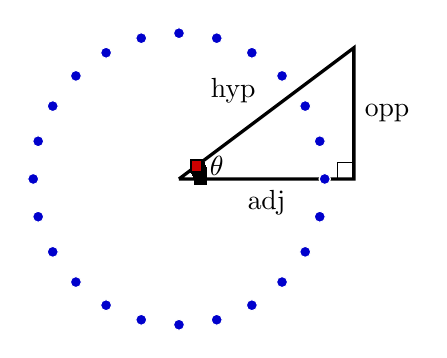
\begin{tikzpicture}
      \begin{axis}[xmax=1.2, axis equal=true, axis lines=none,
        width=2.75in, clip=false]
        \pgfmathsetmacro{\angle}{asin(3/5)};
        \addplot+[domain=0:360, white] ({cos(x)}, {sin(x)});
        \draw[very thick] (0,0) -- node[midway, below] {adj} (1.2, 0) -- node[midway, right] {opp} (1.2, 0.9) -- node[midway, above left] {hyp} (0,0);
        \addplot+[domain=0:\angle, semithick, black] ({.15*cos(x)},
        {.15*sin(x)}) node[pos=0.5, anchor=200] {$\theta$};
        \draw (1.2, 0) rectangle ++(-6pt, +6pt);
      \end{axis}
    \end{tikzpicture}
\end{document}